\documentclass{sig-alternate-05-2015}

\usepackage{amsmath}
\usepackage{amssymb}
\usepackage{hyperref}
\usepackage[utf8]{inputenc}
\usepackage{pifont}
\newcommand{\cmark}{\ding{51}}
\newcommand{\xmark}{\ding{55}}
\newcommand{\specialcell}[2][c]{%
         \begin{tabular}[#1]{@{}c@{}}#2\end{tabular}}

\begin{document}
%\doi{}
%\isbn{123-4567-24-567/08/06}
\title{Improving Topic Models with Word Embeddings and vice versa}
\subtitle{Master Thesis Expos\'e}

\numberofauthors{1}
\author{
\alignauthor
Stefan Bunk\\
       \affaddr{Hasso Plattner Institute, University of Potsdam}\\
       \affaddr{Prof.-Dr.-Helmert-Str. 2-3}\\
       \affaddr{14482 Potsdam, Germany}\\
       \email{stefan.bunk@student.hpi.uni-potsdam.de}
}
\date{9 June 2016}

\maketitle
% \begin{abstract}
% Recently, distributed representations of words, called word embeddings, have gained traction for tasks such as .
% The master thesis will investigate
% \end{abstract}

\section{Introduction}
A core task in natural language processing (NLP) is to understand the meaning of words.
Many downstream NLP tasks profit from this, for example, text categorization, part-of-speech tagging, and machine translation.
A popular concept to qualify the meaning of a word is to look at the contexts, in which the word appears.
A famous quote by Firth says: ``You shall know a word by the company it keeps''~\cite{Firth1957}.
This assumption is also known as the distributional hypothesis.

Two existing approaches in this area are topic modeling and word embeddings.
Topic modeling assumes, that an author has certain topics in mind when writing a document, which are chosen beforehand.
For example, an author could decide to write a document about \emph{politics} (70~\%) in \emph{sports} (30~\%) and then picks the words ``coalition'', ``election'' and ``corruption'' for \emph{politics} and the words ``soccer'' and ``ball'' for \emph{sports}.
Topic modeling techniques, with Latent Dirichlet Allocation being the most popular one, try to recover the hidden topics in large corpora, i.e.\ find out that ``soccer'' and ``ball'' come from the same topic.
As topic models are probabilistic models and hence provide probability distributions as the result, the topics can be easily interpreted by humans.

In word embedding, each word is assigned a vector in a high-dimensional vector space.
These vectors are automatically learned using neural networks.
During the supervised training, each word must try to predict its surrounding words.
This way, the context of a word is encoded in the vector representation of a word.
Using a clever network architecture, these vectors exhibit interesting properties.
First, similar words tend to be in similar positions in the vector space.
For example, when looking for the most similar words for ``France'' using cosine distance, the model outputs ``Spain'', ``Belgium'', ``Netherlands'' and ``Italy''.
Second, the word vectors exhibit interesting linear relationships.
For example, when calculating the vector $vector("King") - vector("Man") + vector("Woman")$ and looking for the closest word at the vector result, the result is the word ``queen''~\cite{Mikolov2013b}.

The two approaches have different origins.
Word embeddings have their roots in the neural network and deep learning community, while topic modeling stems from information retrieval and Bayesian statistics.
% https://www.gavagai.se/blog/2015/09/30/a-brief-history-of-word-embeddings/ THIS BLOG POST IS VERY ENLIGHTENING, GIVES A GOOD OVERVIEW
% These different contextual representations capture different types of semantic similarity; the document-based models capture semantic relatedness (e.g. “boat” – “water”) while the word-based models capture semantic similarity (e.g. “boat” – “ship”). This very basic difference is too often misunderstood.
Hence, there is relatively little research in combination of these two methods.
In this master thesis, we aim to explore potential synergies between these technologies.
In particular, it might be useful to investigate ``whether the two types of models are complementary in the errors they make, in which case combined models could be an interesting avenue for future work''~\cite{Baroni2014}.

This expos\'e is organized as follows: Section~\ref{sec:related-work} will introduce topic modeling and word embeddings, compare the two approaches and show existing work in combining the two methods.
Section~\ref{sec:comparative-evaluation} will present first experiments, which we want to conduct at the start of this master thesis.
Section~\ref{sec:approach} will show our approach for this master thesis.
% Section~\ref{sec:data-sets-and-evaluation} will show different data sets and evaluation tasks to evaluate systems based on topic modelling and word embeddings.

\section{Related Work}
\label{sec:related-work}
\subsection{Topic Modeling}

Many methods for modeling natural language text have been proposed.
An early popular method was tf-idf~\cite{SparckJones1972} scheme, which reduced each document in a corpus to a vector of term frequencies normalized by inverse document frequencies.
Later, Latent Semantic Analysis (LSA)~\cite{Deerwester1990} was proposed to reduce the large matrix to a smaller subspace using singular value decomposition.
While these approaches have their origins in linear algebra, topic models have been developed from a probabilistic view to allow better interpretation.
Topic models are generative probabilistic models of a document collection, which assume hidden topics have guided the generation of the text.
In this way of thinking, an author picks certain topics to write about, and then picks words associated with these topics for a concrete document.
The goal is then to uncover the unseen, so called ``latent'', topics from a text corpus.
All of these approaches have in common, that they assume a bag-of-words representation of documents.

\subsubsection{Earlier approaches}
A basic generative topic model is the mixture of unigrams model~\cite{Nigam2000}.
In this model, a topic is a fixed probability distribution over the vocabulary.
However, only one topic is allowed per document, which limits its predictive power.

A more sophisticated topic model is the probabilistic latent semantic analysis (pLSA), which allows multiple topics per document.
The model is fitted with an Expectation-Maximization algorithm.
However, pLSA does not provide a full generative model applicable to unseen documents.
Also, as the number of parameters grows linearly with the number of training documents, it tends to overfit~\cite{Blei2003}.

\subsubsection{Latent Dirichlet Allocation (LDA)}
LDA was proposed by Blei et al.~\cite{Blei2003} for modeling text corpora and other collections of discrete data.
In an unsupervised fashion, it can automatically detect similarities between words and group them in one topic.
The number $K$ of topics is constant and must be chosen beforehand.
% TODO thesis: Add nice example document with figure, e.g. k=3 and some topics

LDA defines a topic as a distribution over a fixed vocabulary.
Different topics assign different probabilities to the same word, for example, the word ``soccer'' would have a much higher probability in a \emph{sports} topic than in a \emph{politics} topics.
The opposite would hold for the word ``coalition''.
Note that a topic is only a distribution over words, i.e.\ LDA does not generate a name or a summary for a topic.

A document is assumed to consist of one or several topics with a certain, fixed distribution.
A document could be $20~\%$ about \emph{sports} and $80~\%$ percents about \emph{politics}, or $30~\%$ about \emph{climate}, $25~\%$ about \emph{cars} and $45~\%$ about \emph{politics}.
In general, LDA aims to generate sparse distributions for both cases, i.e.\ a topic should have only a few words (relative to the vocabulary of the entire corpus) with high probability and a document should have only a few topics.
This is governed by two scalar hyperparameters $\alpha$ and $\beta$, which influence two symmetrical prior Dirichlet distributions.

With these two hyperparameters, the generative document creation process of LDA can be summarized as follows:
\begin{enumerate}
       \item Fix number of topics $K$ in the document collection
       \item Choose word distributions $\phi_j \sim Dirichlet(\beta)$ for each topic $j \in \{1~..~K\}$
       \item Now, for each document $d$:
       \begin{enumerate}
              \item Choose topic distribution $\theta_d \sim Dirichlet(\alpha)$
              \item For each position $i$ in the document
              \begin{enumerate}
                     \item Choose topic $z_{d,i} \sim Multinomial(\theta_d)$
                     \item Choose word $w \sim Multinomial(\phi_{z_{d,i}})$ for current word
              \end{enumerate}
       \end{enumerate}
\end{enumerate}
This process is also illustrated in the probabilistic graphical model in plate notation in Figure \ref{fig:lda}.
This model can also be seen as a soft-classification of documents: instead of assuming exactly one topic per document, each word in a document can potentially come from a different topic.

\begin{figure}
       \centering
       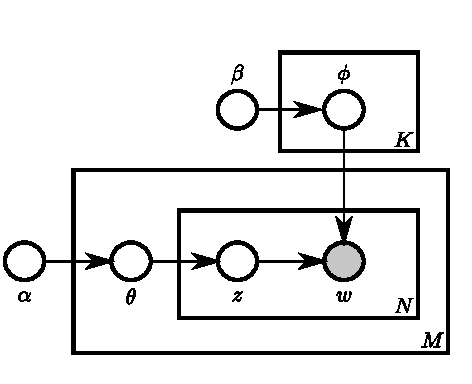
\includegraphics{figures/lda.pdf}
       \caption{Graphical model for Latent Dirichlet Allocation with $K$ topics, $M$ documents and $N$ words in a document.}
       \label{fig:lda}
\end{figure}

In reality, we only observe the words in the documents, and need to reverse engineer the hidden, ``latent'' parameters of the model, namely the word distribution per topic $\phi$, the topic distribution per document $\theta$ and the word-topic assignments $z$.
In this process, called \emph{inference}, we try to find the most probable parameter assignments, which could have generated our document collection.
Computationally, this is equivalent to finding the posterior distribution of the parameters given the observed words.
Blei et al.~\cite{Blei2003} propose an algorithm based on variational approximation, however Griffiths and Steyvers~\cite{Griffiths2004} proposed an algorithm based on Gibbs sampling, which is more popular nowadays.
% expand here: limiting distribution, sampling formula etc.

The output of running LDA on a corpus is three-fold:
\begin{itemize}
       \item Topics as set of similar words, e.g.\ the terms ``soccer'', ``ball'', ``league'' could form a topic named \emph{sports}.
       \item Topic distribution of a single word, e.g.\ the term ``jaguar'' occurs 80~\% in the \emph{cars} topic and 20~\% in the \emph{animals} topic
       \item Topic distribution inside a concrete document or inside the entire corpus
\end{itemize}

LDA has been applied to many domains, namely document modeling, text classification, collaborative filtering~\cite{Blei2003} and document summarization~\cite{Wang2009}.
Other use cases include population genetics~\cite{Pritchard2000} and computer vision~\cite{LiFei-Fei2005}.

\paragraph{Implementations}
There exist implementations of LDA in Java, C/C++, Python and Matlab.
In this thesis, we will use two particularly fast and robust implementations:
\begin{itemize}
       \item Mallet by McCallum~\cite{McCallum2002}, Java
       \item gensim by {\v R}eh{\r u}{\v r}ek~\cite{Rehurek2010}, Python
\end{itemize}

% LDA has problems on small texts/documents

\subsection{Word Embeddings}

In traditional language modeling, words are treated as atomic units by a discrete one-hot encoding.
Given a vocabulary $V$, each word $w$ is assigned a vector of length $|V|$ with all values set to zero except one to uniquely identify the word.
A typical architecture involves n-grams, which try to predict the next word based on previous words.
This approach has two disadvantages.
First, it limits the context to an arbitrary range.
When n is too small, only the immediate preceding words are taken into account, failing to capture long-range word dependencies.
When n is too large, the \emph{curse of dimensionality} becomes a problem: when representing a joint sequence of $n$ words, there are $|V|^n$ potential combinations.
As most n-grams are never observed, this leads to very sparse vectors.
Second, this type of language modeling does not capture similarity between words and also does not capture information about the relationship between words.
When using the one-hot encoding, both the words ``house'' and ``houses'' get a unique vector with no indication of similarity.
If one would employ cosine distance or euclidean distance to assess similarity in the vector space, all words would be equally similar.

In contrast to this, the idea of \emph{distributed representations} is to not represent objects by discrete counts but rather by continuous points in a vector space $\mathbb{R}^m$, where $m$ is much smaller than $|V|$.
The idea of distributed representations has a long history, dating back to the mid-eighties with work from Hinton and Rumelhart~\cite{Hinton1986,Rumelhart1988}.
Intuitively, instead of using one dimension for each atomic unit, distributed representations assign meanings to the dimensions and then recombine these meanings for a concrete object.
%For example to represent , one dimension could indicate the size of an object, another one the color.
%With just three dimensions, one could represent small 
%If one dimension indicates how green an object is and another dimension indicates whether an object is a flower, then one could represent a green flower with high values in both dimensions instead of requiring one dimension for red, blue, and green flowers.
Recently, the term \emph{word embeddings} was also used to describe the approach of embedding words in a vector space.
We will use the terms \emph{distributed representation}, \emph{word vectors} and \emph{word embeddings} interchangeably in this document.

The use of distributed representations for words was proposed by Bengio et al.~\cite{Bengio2003}.
In their work, they train a neural network to predict a word given the preceding context.
This prediction model is again based on the distributional hypothesis: words are similar, if they occur in the same contexts.
With this architecture, ``the system naturally learns to assign similar vectors to similar words''~\cite{Baroni2014}.
%https://en.wikipedia.org/wiki/Distributional_semantics#Distributional_Hypothesis

In a series of papers, Mikolov et al.~\cite{Mikolov2013,Mikolov2013a,Mikolov2013b} provided a better neural architecture to train the word vectors.
Contrary to the trend of ever deeper models, a shallower model with no hidden layer was more successful in building better word vectors, because it can be trained on more data.
As Mikolov et al.~\cite{Mikolov2013a} state, ``it might not be able to represent data as precisely as neural networks, but can possibly be trained on much more data efficiently.''
Due to the state-of-the-art performance and the free open source implementation \emph{word2vec}\footnote{\url{https://code.google.com/archive/p/word2vec/}} this method gained popularity and will also be used in this thesis.

Mikolov et al.\ presented two models.
The continuous bag-of-words model (CBOW) works by predicting the center word in a symmetric context window.
The continuous skip-gram model works the other way round: given a word, it tries to predict the context.
We focus on the skip-gram model in the following, as it had the better evaluation results in the original paper.
In the skip-gram model, surrounding words have to be encoded in the word vector for each word or as Mikolov et al.~\cite{Mikolov2013} state ``vectors can be seen as representing the distribution of the context in which a word appears''.
% TODO: Skip-Grams with Negative Sampling

A nice property of the trained word vectors is, that linear relationships between words are kept in the vector space.
It was shown that
\begin{center}
       $vector("King") - vector("Man") + vector("Woman")$
\end{center}
is closest to the vector representation of the word ``queen''~\cite{Mikolov2013b}.
Interestingly, this relationship holds for both semantic and syntactic similarly~\cite{Mikolov2013a}, such as
\begin{center}
       $vector("houses") - vector("house") + vector("car")$
\end{center}
is closest to $vector("cars")$.
% Quote from webpage: This seems to be a great strength of neural networks: they learn better ways to represent data, automatically. Representing data well, in turn, seems to be essential to success at many machine learning problems. Word embeddings are just a particularly striking example of learning a representation.

Word embeddings have been used in many natural language and machine learning tasks.
They are a natural input to many machine learning algorithms, as they provide a better encoding than the traditional one-hot encoding.
Concrete use cases involve statistical language modeling, machine translation~\cite{Zou2013}, sentiment analysis~\cite{Maas2011} and paraphrase detection.

\paragraph{Implementations}
The original implementation of the approach by Mikolov et al.~was open sourced under the name \emph{word2vec}.
It is implemented in C and can be used as a command line tool.
There also exists another implementation in the gensim package by {\v R}eh{\r u}{\v r}ek~\cite{Rehurek2010}.
These two implementations can run multi-threaded in the CPU.
There also exist some GPU implementations, however, these are not as stable.
Therefore, we will concentrate on the CPU implementations first.

\subsection{Comparison between LDA and Word Embeddings}

At their foundations, LDA and word embeddings come from different backgrounds.
LDA stems from Bayesian statistics, while word embeddings were first developed in the neural-network and deep learning community.
Baroni et al.~\cite{Baroni2014} show, that both methods fundamentally are based on the assumption that ``semantically similar words tend to have similar contextual distributions''.
However, the methods use this base hypothesis to come to different conclusions.
%LDA and word embeddings have different underlying assumptions about the text.
LDA works on the bag of words assumption, i.e.\ it treats a document as a whole and does not use the order of the words.
When making a prediction for the next word, LDA makes a global prediction based on the topic distribution in the current document.
Word embeddings, on the other hand, generate the next word based on the context of the word and are per se local.
%Word embeddings are per se local as they try to predict the immediate context of a word.

Both LDA and word embeddings can provide distributed representations for words.
In LDA, this works by taking the topic distribution for a word as the embedding in the topic space.
However, this representation is not good at keeping linear relationships~\cite{Mikolov2013b,Mikolov2013a}.
Also, it tends to yield sparse vectors as LDA tries to keep the number of topics per word small.

Baroni et al.~\cite{Baroni2014} also introduce the classification of count-based methods and prediction-based methods in distributional semantic models.
Prediction-based methods try to set word vectors so that they are able to predict the context words.
Count-based methods are based on counting the occurrence of words and co-occurrence with other words.
Popular count-based methods typically use pointwise mutual information (PMI) and matrix transformation on the co-occurrence matrix.
While word embeddings are clearly a prediction-based method, LDA constitutes a hybrid type in this classification.
LDA is based on word counts and co-occurrences and treats words as discrete observations, however, the model parameters are chosen to maximize its predictive power.

Another aspect is the interpretability of the model.
LDA forces the elements in a vector to sum up to 1 and all values must be non-negative.
Thus, the embedding of a word in the topic space is easily interpretable by humans.
With a word vector of $[0~0~0.2~0.8]$ and given the meanings of a topic, a word can be interpreted as being used $20~\%$ in \emph{sports} and $80~\%$ in \emph{politics}.
When working with word embeddings, a vector like $[{-2.4}~0.3~1.3~{-0.1}]$ is not interpretable.
The arbitrary dimensions and values of a word embedding vector cannot be understood by humans.

Regarding the performance, LDA operates much slower than word embeddings.
LDA becomes very expensive on large data sets, because it needs to repeatedly iterate over the entire corpus.
The method by Mikolov has been successfully trained on a corpus with about 100 billion words.

% TODO: both somewhat use vector space model TODO: add seminal reference
% distributional semantic models (DSMs)

\subsection{Existing combinations}
The existing related work, which combines topic modeling approaches with word embeddings, can be roughly divided in two directions.
One type of model tries to improve topic models by incorporating word vectors, while the other aims to improve word embeddings with topic models.
We summarize the prior work in this field in Table~\ref{table:tm_and_we_combinations}\footnote{ToCoh: Topic Coherence, WordSim: Word Similarity, DocClass: Document Classification, DocClust: Document Clustering, Analogy: Word Analogy Reasoning, SentComp: Sentence Completion}.
\begin{table*}
       \centering
       \caption{Overview over related work of combinations between topic models (TM) and word embeddings (WE) and how they have been evaluated}
       \begin{tabular}{|l||c|c||c|c|c|c|c|c|}
              \hline
              \textbf{Paper}                  & \textbf{TM} & \textbf{WE} & \textbf{ToCoh} & \textbf{WordSim} & \textbf{DocClass} & \textbf{DocClust} & \textbf{Analogy} & \textbf{SentComp} \\
              \hline
              Blei et al.~\cite{Blei2003}     & \cmark &  &                &                  & \specialcell{\cmark\\\textsc{Reuters}}  &                   &  & \\
              \hline
              Mikolov et al.~\cite{Mikolov2013a} &     & \cmark &                &           &                      &                   & \cmark & \specialcell{\cmark\\\textsc{Microsoft}\\\textsc{sentence}\\\textsc{completion}} \\
              \hline \hline
              Das et al.~\cite{Das2015}       & \cmark &  & \specialcell{\cmark\\Wikipedia\\co-occurrence} &      &                   &                   & & \\
              \hline
              Nguyen et al.~\cite{Nguyen2015} & \cmark &  & \specialcell{\cmark\\Wikipedia\\co-occurrence} &      & \specialcell{\cmark\\\textsc{20-News-}\\\textsc{Group},\\\textsc{TagMyNews}} & \specialcell[h]{\cmark\\Same as\\left} & & \\
              \hline
              Sridhar~\cite{Sridhar2015}      & \cmark &  & \specialcell{\cmark\\Manual\\annotation}               &                  &                   &  & & \\
              \hline
              Moody~\cite{Moody2016}          & \cmark & \cmark & \specialcell{\cmark\\Palmetto\footnotemark\\evaluation tool}         & \specialcell{\cmark\\Only\\qualitative} &                      &         & & \\
              \hline
              Liu et al.~\cite{Liu2015} &     & \cmark &                & \specialcell{\cmark\\\textsc{SCWS}}    & \specialcell{\cmark\\\textsc{20-News-}\\\textsc{Group}}               &                   &  & \\
              \hline
              Cheng et al.~\cite{Cheng2015} &     & \cmark &                & \specialcell{\cmark\\\textsc{SCWS} +\\paraphrase\\detection\\\textsc{MSRPC}}    &  &                   &  & \\
              % • Nguyen et al.~\cite{Nguyen2015}} & • \parbox[t]{7cm}{Conceptual Text Understand in Distributional Semantic Space, Cheng et al.~\cite{Cheng2015}} \\
              % • \parbox[t]{7cm}{Unsupervised Topic Modelling for Short Texts Using Distributed Representations of Words, Sridhar~\cite{Sridhar2015}} & • lda2vec, Moody~\cite{Moody2016} \\
% • Topical Word Embeddings, Liu et al.~\cite{Liu2015}
              \hline
       \end{tabular}
       \label{table:tm_and_we_combinations}
\end{table*}
\footnotetext{The online evaluation tool can be accessed at \url{http://palmetto.aksw.org/palmetto-webapp}}
% \begin{table*}
%        \centering
%        \caption{Overview over related work of combinations between topic models and word embeddings}
%        \begin{tabular}{|l|l|}
%               \hline
%               \textbf{Output: Topic Model} & \textbf{Output: Word Embeddings} \\
%               \hline
%               • Gaussian LDA, Das et al.~\cite{Das2015}                                                          & • Topical Word Embeddings, Liu et al.~\cite{Liu2015} \\
%               • \parbox[t]{7cm}{Improving Topic Models with Latent Feature Word Representations, Nguyen et al.~\cite{Nguyen2015}} & • \parbox[t]{7cm}{Conceptual Text Understand in Distributional Semantic Space, Cheng et al.~\cite{Cheng2015}} \\
%               • \parbox[t]{7cm}{Unsupervised Topic Modelling for Short Texts Using Distributed Representations of Words, Sridhar~\cite{Sridhar2015}} & • lda2vec, Moody~\cite{Moody2016} \\
%               \hline
%        \end{tabular}
%        \label{table:tm_and_we_combinations_previous}
% \end{table*}

The work by Das et al.~\cite{Das2015} belongs to the first group. They propose a method named Gaussian LDA.
In this approach, a topic is no longer a distribution over words in the vocabulary, but a Gaussian distribution in the word embedding space.
Also, words are no longer atomic units, but are represented by their corresponding pre-trained word embeddings.
Each topic is associated with a mean $\mu_k$ and a covariance matrix $\Sigma_k$.
The prior distribution over the means is a normal distribution, and the prior distribution over the covariances is an inverse Wishart distribution.
These parameters are inferred using Gibbs sampling as in standard LDA. % together with linear algebra tricks
Another idea is proposed by Sridhar~\cite{Sridhar2015}.
They start by training word embeddings.
Afterwards they fit a Gaussian mixture model directly on the word embedding space.
A topic is represented by mean and covariance matrix.
In contrast to Das et al.~\cite{Das2015}, Sridhar~\cite{Sridhar2015} assumes the topics to be fixed given the word embeddings, while Das et al.~\cite{Das2015} only take the embeddings as a basis and still learn the topics based on the word co-occurrences in the corpus.
Another approach is taken by Nguyen et al.~\cite{Nguyen2015}.
They use word embeddings, ``latent feature word representations'' in their words, to sample words not only from the multinomial topic distribution, but also from the embedding space.
Instead of directly sampling a word from the topic-word distribution of the chosen topic, they introduce a Bernoulli parameter $s \sim Ber(\lambda)$.
This parameter decides, whether the word is sampled as usual from the topic-word distribution or from the latent feature vectors.
To sample in the embedding space, they sample from a softmax-normalized categorical distribution defined by:
\begin{equation*}
       Cat(w | \tau_t, \omega) = \frac{exp(\tau_t * \omega_w)}{\sum_{w' \in W} exp(\tau_t * \omega_{w'})},
\end{equation*}
where $\tau_t$ is the representation of topic $t$ in the word embedding space and $\omega$ are the pretrained and fixed word embedding vectors.
The authors use pretrained vectors from \emph{word2vec}~\cite{Mikolov2013a} and \emph{GloVe}~\cite{Pennington2014}.
The topic embeddings $\tau$ are updated in each iteration of Gibbs sampling via a MAP estimate based on all other parameters given.
A similar idea is used by Cheng et al.~\cite{Cheng2015}.
In fact, the first model they propose is the same as the first model from Nguyen et al.~\cite{Nguyen2015}.
In addition to some other new models, which are similar to Cheng et al.'s work, they also propose new models, which do not assume independence between word and concept embeddings.
These \emph{generative word-concept skip-gram} models perform best in their word-similarity and paraphrase detection benchmarks.

We now focus on methods for better word embeddings.
Liu et al.~\cite{Liu2015} propose Topical Word Embeddings.
These embeddings make use of word topics inferred via LDA to generate better word vectors.
They propose three different architectures.
The first method regards topic as pseudo words, which are added to the context of each word.
Thus, an embedding for a word and its topic is learned independently.
The second method considers each pair of word and topic as a pseudo word.
The third method works the same way, except that it learns only one word embedding vector per word and one topic embedding vector per topic.
These two vectors are then combined for the vector of the word-topic pair.
To the authors' surprise, the simplest method one performs best in their word similarity and text classification benchmarks.
Using the additional topic information when training word embeddings has practical benefits for similarity evaluation.
When the model is asked for similar words to the word ``apple'', it returns ``peach'', ``juice'', ``strawberry'' or it returns ``mac'', ``ipod'', ``android'' depending on the topic of the word.

Moody~\cite{Moody2016} proposes lda2vec.
His method learns word vectors together with learning topic vectors and an intuitive topic-based document interpretation.
Even though trained in the word embedding space, the topic-document vectors are still kept parse to be interpretable for humans.
However, the method is not evaluated extensively and it is unclear, whether this method yields improved word vectors.

% FROM MIKOLOV COLING 2014 tutorial
% Sentence-level representations
% • To obtain sentence level representations, we can add unique tokens
% to the data, one for each sentence (or short document)
% • These tokens are trained in a similar way like other words in the skipgram
% or CBOW models, just using unlimited context window (within
% the sentence boundaries)

A word vector can be seen as a summary of the word with all its meanings.
Many applications require not only word vectors, but also summaries of longer chunks of text.
Therefore, it is necessary to embed sentences or documents in the word embedding space.
For this problem, Le and Mikolov~\cite{Le2014} proposed paragraph vectors.
In their work, paragraph can mean an arbitrary long text, ranging from sentences to entire documents.
Paragraph vectors are trained by adding an artificial word to each context, which represents the current paragraph.
These paragraph vectors can then be viewed as a summary of the meaning of the entire paragraph, which is useful for further downstream applications.
%for sentiment analysis by training logistic regression classifier on the vectors.
% http://sentic.net/sentire2011ott.pdf

%one is supervised, the other one is unsupervised

%``A long tradition in computational linguistics has shown that contextual information provides a good approximation to word meaning, since semanti- cally similar words tend to have similar contex- tual distributions (Miller and Charles, 1991).''
%``It remains to be seen whether the two types of models are complementary in the errors they make, in which case combined models could be an interesting av- enue for further work.''
%there has been a shift from the LDA to the word embeddings


% \begin{itemize}
       % \item
       %        Directly run a GMM on the word embedding space --> See Gaussian LDA
       % \item
       %        Run LDA first.
       %        Then run word embedding training, except that the word also has to predict the surrounding context.
       %        Problem: LDA performance
       % \item
       %        Run LDA first.
       %        Then run word embedding training, except that the same word from different topics gets a unique token
       %        Problem: LDA performance
       % \item
       %        Try to interpret word embedding dimensions using topic models.
       %        This requires a labelled topic model, i.e.\ topic 40 is about sports.
       %        Then try to put a label on a word embedding dimension, for example, the large the value in dimension x the more about sports.
       % \item
       %        Run LDA, then calculate average word vector and covariance matrix for all topics.
       %        Check, how well the topics are distributed in the topic space.
       %        This also allows to assign unseen words to a topic.
% \end{itemize}

% \subsection{Preprocessing}
% No-stemming (does harm in both \emph{word2vec} and topic modelling), as it destroys the difference between Apple and apples and (TODO: other example) as well as small/smallest.
% Quoting lots of stuff from the lda2vec

% \subsection{Enhancing topic models?}
% Then we need evaluation for topic models and show that they are better
% Use pretrained word vectors to improve~\cite{Das2015}


\section{Comparative Evaluation of Existing Approaches}
\label{sec:comparative-evaluation}
In the master thesis, we will start with a comparative evaluation of word embeddings and topic models.
As shown in Table~\ref{table:tm_and_we_combinations} there is no evaluation strategy for the different models.
There is a wide range of tasks, which we can use to evaluate and compare different approaches.
We build on the following set of evaluation tasks, ranging from low-level, artificial tasks to higher-level use cases:
\begin{itemize}
       \item
              \emph{Word Similarity}:
              Word similarity can be measured for models, which output word embeddings.
              We will use the Stanford Contextual Word Similarity data set (\textsc{SCWS}) by Huang et al.~\cite{Huang2008}.
              This data set evaluates word similarity given the context of the word.
              For example, ``bank'' might be similar to the word ``money'', when used in the context ``My \emph{bank} account number is 123.'', but not when used in the context ``the east \emph{bank} of the river''.
              We will also use the \textsc{WordSim-353} data set by Finkelstein et al.~\cite{Finkelstein2002}, which judges the similarity of words without a context.
              It will be interesting to see whether the topic-model-enhanced word embeddings have better improvements on the SCWS data set than the standard model.
% \subsection{Topic Coherence}
% Standard method to evaluate topic models: measure the likelihood of held-out documents.
% Another approach to evaluate the topic coherence is to compute the Pointwise Mutual Information of the top $k$ words of a topic with co-occurrence counts from Wikipedia.
       \item
              \emph{Topic Coherence}:
              This is the standard evaluation for topic models.
              We will build on the work by Röder et al.~\cite{Roder2015}.
              They evaluate more than 200,000 coherence measures on several data sets, and determine the coherence measure with the highest correlation to human-annotated coherence ratings.
              We will use their results to decide on a topic coherence measure for our evaluations.
       \item
              \emph{Concept Categorization}:
              This task can be done by both topic models and word embeddings.
              The task is to sort instances of an abstract entity into the same category.
              For example, both the terms ``chicken'' and ``dog'' or ``car'' and ``boat'' should be in the same category, as both are ``animals'' and``vehicles'', respectively.
              We will use two existing data sets for this task.
              The first one from the ESSLLI 2008 Distributional Semantic Workshop contains 44 words in 6 categories.
              The second data set from Baroni et al.~\cite{Baroni2010} includes 83 words from 83 words in 10 categories.
       \item
              \emph{Sentence Completion}:
              The Microsoft Research Sentence Completion Challenge~\cite{Zweig2011} consists of 1,040 sentences, in which one word is missing.
              Five options are offered for the missing word, and an algorithm must decide, which one fits best.
              This is a natural task for word embeddings, as they are trained on exactly that task.
              It is also a task, where topic models could help achieve better performance, as they could help distinguish between different concepts and topics.
       \item
              \emph{Document Classification}:
              We will use two standard text classification data sets, namely the \textsc{Reuters-21578} data set (8,000 documents) and the \textsc{20-News-Group} (20,000 documents) data set.
       \item
              \emph{Information Retrieval}:
              Wei et al.~\cite{Wei2006} proposed an approach to use LDA in information retrieval.
              We will evaluate the different LDA adaptions using this approach on different TREC data sets.
              We will also conduct further research, how word embeddings are used in information retrieval.
              % OHSUMED
       \item
              \emph{Other Applications}: We will investigate other use cases, which can be used for evaluation, for example sentiment analysis or recommendation tasks.
% OTHER IDEAS:
% \subsection{Concept categorization}
% Cluster words, measure cluster purity
% Sentiment Analysis
% \cite{Wei2006}
%\paragraph{Document Clustering}
% Not particular useful, as they do different things
% \paragraph{Sentiment Analysis}
% \subsection{Catch out of the list words?}
% Given a word, find the word, which does not fit in the list.  % data set?
% \paragraph{Language Modelling}
% Blei et al.~\cite{Blei2003} present ... We use perplexity as our evaluation metric.
% This is out, as LDA is no language modelling technique. Word embeddings will win.

\end{itemize}
These evaluation task list will probably be adapted and changed throughout the thesis.
The list of approaches for evaluation also depends on the availability of the code for the respective systems.
We estimate this evaluation to take two months.

\section{Approach}
\label{sec:approach}

In the master thesis, we try to find ways of combining word embeddings and topic modeling.
We will start with a set of experiments to explore both base methods and to work out their differences:
\begin{itemize}
       \item
              \emph{Visualize similar words in topic space}:
              We will train word vectors using \emph{word2vec} on the English Wikipedia.
              Similarly, we will apply LDA on the same corpus to compute topics.
              Then, using cosine similarity for comparing vectors, we will identify similar words in the word embedding space.
              Using these data, we can compare how much similar words overlap with topics from the LDA model.
              % Plot: Similarity threshold vs. "topicness"/topic overlap. The lower the similarity threshold, the higher should be the topic overlap.
       \item
              \emph{Visualize words from one topic in embedding space}:
              Again, we will train \emph{word2vec} and apply LDA to the English Wikipedia.
              Using dimensionality reduction techniques like t-SNE~\cite{VanDerMaaten2008} or Principal Component Analysis, we can project the high-dimensional embedding space down to a two-dimensional map.
              It will be interesting to see whether the words from one topic cluster in similar regions in the two-dimensional embedding map.
\end{itemize}

These experiments will also help set up the code and infrastructure for further experiments during the master thesis.
We estimate these experiments to take two weeks.

Next, we plan to experiment with a new combination of word embeddings and topic models.
We currently believe, that a new LDA-model incorporating the word embeddings in the sampling process is the most promising direction for further research.
Concretely, we plan to work on short documents.
Plain LDA usually has problems finding good topics in short documents, because there are only a few co-occurrences of words.
In this case, it could help to use word embeddings to make use of similar words.
To achieve this, we plan to have a deeper look at the work of Nguyen et al.~\cite{Nguyen2015}.
We will reimplement their approach and try to find improvements using our background from the experiments and the comparative evaluation.
This part of the master thesis will take estimated two months.

To summarize our approach to the master thesis, we will start with experiments to work out the differences between topic models and word embeddings.
Then we will work on two work streams in parallel.
One, we will evaluate existing systems to find out their weaknesses and strengths.
Second, we will reimplement the paper by Nguyen et al.~\cite{Nguyen2015} and try to improve from there.

% \section{Data Sets}
% \label{sec:data-sets-and-evaluation}

% %For the evaluation we prefer tasks, which can be performed by both topic models and word embeddings, so we can compare the performance of different joint systems.
% % https://cloud.google.com/bigquery/public-data/hacker-news#exploring_the_data_using_looker

% Both LDA and word embedding require large amount of text data.
% Unfortunately, the offical data set for \emph{word2vec}, a compilation of 100 billion words from Google News, is not publicly available.
% Thus, we will use other text corpora in this master thesis to train topic models and word embeddings.
% \begin{itemize}
%        \item
%               \textsc{Wikipedia}:
%               The full text of the English Wikipedia is available as an XML data dump.
%               We will focus on this data set first as it is reasonably sized, well known and covers a wide range of general topics.
%        \item
%               \textsc{CommonCrawl}:
%               This data set includes full web pages and text extractions from 7 years of crawling the web.
%               This data set is much bigger than \textsc{Wikipedia} and will be used, if larger scale experiments are needed.
%        \item
%               \textsc{Hacker News comments}:
%               This corpus contains 75 million tokens in 66 thousand documents with 110,000 unique tokens.
%               It is interesting, because it contains news about a specialialized topic, which are only interesting too a small group of people.
%               The topics in this corpus are expected to be significantly different than standard topics in news data sets.
%        % \item
%        %        \textsc{1 Billion Word Language Model Benchmark}:
%        % \item
%        %        ukWaC: 2 billion word corpus constructed from web crawling limited to .uk domain
%        % \item
%        %        \textsc{British National Corpus}: 100 million word collection of written and spoken English language from the 1980s and 1990s, requires application
% \end{itemize}


% \section{Conclusion}
% \label{sec:conclusion}
% In this master thesis, we will investigate methods


\bibliographystyle{abbrv}
\bibliography{expose}
\end{document}

